% don't remove the folling lines, and edit the defintion of \main if needed
\documentclass[../report.tex]{subfiles}
\providecommand{\main}{..}
\IfEq{\jobname}{\currfilebase}{\AtEndDocument{\biblio}}{}
\IfEq{\jobname}{\currfilebase}{%file for shortcuts

\newcommand{\nch}{\ensuremath{N_{\mathrm {ch}}\xspace}}
\newcommand{\Ncoll}{\ensuremath{N_{\mathrm {coll}}}}
\newcommand{\Npart}{\ensuremath{N_{\mathrm {part}}}}
\newcommand{\dNdeta}{\mathrm{d}N_\mathrm{ch}/\mathrm{d}\eta}
\newcommand{\snn}         {\ensuremath{\sqrt{s_{\mathrm {NN}}}}}
\newcommand{\kT}          {\ensuremath{k_{\mathrm {T}}}}

\newcommand{\pp}          {pp}
\newcommand{\pPb}         {pPb}
\newcommand{\pA}          {pA}
\newcommand{\PbPb}        {PbPb}
\newcommand{\AuAu}        {AuAu}
\newcommand{\CuCu}        {CuCu}
\newcommand{\pAu}         {pAu}
\newcommand{\dAu}         {dAu}
\newcommand{\lsim}        {\,{\buildrel < \over {_\sim}}\,}
\newcommand{\gsim}        {\,{\buildrel > \over {_\sim}}\,}
\newcommand{\co}[1]       {\relax}
\newcommand{\nl}          {\newline}
\newcommand{\el}          {\\\hline\\[-0.4cm]}}{}
% until here


%<Notes>
% Dear contacts,

% Several chapters have started defining custom commands, and this lead to some compilation issues.

% I have now prepared a file commands.tex which is in the main folder. 
% This file is included when you compile the full report (report.tex), but also when you compile the separate sections.

% Please add your custom commands to this file. When you do that, please
% - check that a command does not already exist and can be used,
% - add a comment above your commands, e.g. "% heavy flavour"

% NB. pT is \pT (already predefined in a CERN report style file). Please replace in case you are using \pt

% Best regards,
% Jan Fiete
%</Notes>

% 05/09/18 09:31:59
% Hello John,

% Very good. In addition, we should write explictly in "your" chapter that we decided for the projections to use p = 1.5 ... 1.9 which converts into an increase of LNN of 8 ... 25.

% Best regards,
% Jan Fiete


\begin{document}

\section{Heavy-ion performance of LHC, HL-LHC and HE-LHC}  

\begin{raggedright}
\textbf{Coordinator}: John M. Jowett (CERN)
\linebreak
\textbf{Contributors}: 
Roderik Bruce, John M. Jowett, Michaela Schaumann (CERN),  
Marc A. Jebramcik (Johann-Wolfgang-Goethe Universit\"{a}t, Frankfurt \& CERN) 
 
\end{raggedright} 


\subsection{Heavy-ion performance of LHC in Runs~1 and 2}


This year's 4th one-month Pb-Pb run of the LHC will bring its Run~2 to an end and launch the hardware upgrades to the collider, and to the ALICE experiment, that should allow the full  ``HL-LHC'' heavy-ion performance to be delivered from 2021 onward.   
Indeed, if we compare the specifications of the 2004 LHC Design Report  \cite{lhc1}, for Pb-Pb collisions only with a peak luminosity of \lumival{1}{27},  much  of the upgraded performance is already in hand.   
Not only has that peak Pb-Pb luminosity goal been exceeded by a factor of 3.6, but the p-Pb collision mode---an upgrade beyond the initial design whose very feasibility was widely doubted---has yielded similarly high luminosity 
in multiple operating conditions  (see \cite{Jowett:2018yqk} and references therein). 
Table~\ref{tab:LHCparams} summarises the main parameters of the runs to date. 
Most recently, in 2017, the LHC has collided beams of Xe nuclei \cite{Schaumann:2018qat}, 
providing many of the new results presented in this conference.  
The goal for 2018 will be to complete the accumulation 
of an integrated \PbPb\ 
luminosity of \qty{1}{nb^{-1}} to 
each of the ALICE, ATLAS and CMS experiments.  

	
\begin{table*}[t]
\caption{Representative simplified beam parameters 
at the start of the highest luminosity physics   fills, 
in conditions that lasted for $>\qty{5}{days}$,   
in each annual Pb-Pb and p--Pb run~\cite{ipac2011:Jowett:2011zz,Jowett:1492972,ipac2013:Jowett:1572994,ipac2016:PbPb2015,ipac2017:Jowett:2289686}.  
The original design values for Pb--Pb~\cite{lhc1} 
and p-Pb~\cite{Salgado:2011wc}  
and future upgrade Pb--Pb goals are also shown 
(in these columns the integrated luminosity goal is to be attained over the 4~P--Pb 
runs in the
{10-year periods} before and after 2020).
Peak and integrated luminosities are averages for ATLAS and CMS 
(ALICE being levelled).
The smaller luminosities delivered to LHCb from 2013--2016 and 
in the minimum-bias part of the run in 2016 are not shown.
Emittance and bunch length are RMS values. 
Single bunch parameters for \pPb\ or \Pbp\ runs 
are generally those of the Pb beam.
The series of runs with $\sqrt{\sNN}=\qty{5.02}{TeV}$ also included \pp\ reference runs, not shown here.
Design and record achieved nucleon-pair luminosities are \protect\fbox{boxed}, and some key \pPb\ parameters are 
set in \textcolor{red}{red type}, for easy comparison. 
The upgrade peak luminosity is reduced by a factor $\simeq3$ from its potential value by levelling.
\label{tab:LHCparams}}	
\centering
    {\small
        {\renewcommand{\arraystretch}{1.2}
\begin{tabular}{m{3.7cm}|cc|ccccc|c@{}}
\hline                   
  Quantity                        & \multicolumn{2}{c|}{``design''} & \multicolumn{5}{c|}{achieved} & upgrade \\
  \hline
Year                                & (2004)&(2011)  & 2010 & 2011 &2012--13& 2015 &2016& $\ge$2021 \\
Weeks in physics & - & - & 4 & 3.5& 3 & 2.5& 1, 2 &-\\
Fill no. (best)  & & & 1541 & 2351 & 3544& 4720 &5562& -\\
%circumference $C$   & km            & \multicolumn{5}{c}{ 26.659 } \\
%%mass and charge numbers $A,Z$   & ...  & \multicolumn{3}{c}{--- 208, 82 ---} \\
Species                         &\PbPb &\textcolor{red}{\pPb}& \PbPb&\PbPb & \textcolor{red}{\pPb}& \PbPb &\textcolor{red}{\pPb}& \PbPb \\
Beam energy \qty{E[Z}{TeV]}  & \multicolumn{2}{c|}{ 7 } & \multicolumn{2}{c}{3.5} & 4 & 6.37  & 4,6.5 & 7 \\
Pb beam energy \qty{E[A}{ TeV]}  & \multicolumn{2}{c|}{2.76} & \multicolumn{2}{c}{ 1.38 } & 1.58 &   2.51 & 1.58,2.56  & 2.76 \\
\raggedright Collision energy \qty{\sqrt{\sNN}}{[TeV]}  & 5.52& \textcolor{red}{8.79}& \multicolumn{2}{c}{2.51}& \textcolor{red}{\textbf{5.02}} & \textbf{5.02}& \textcolor{red}{\textbf{5.02},8.16}& 5.52  \\
\hline
Bunch intensity \qty{N_b}{[10^8]}       & \multicolumn{2}{c|}{0.7} & 1.22 &1.07   & 1.2 & 2.0 &2.1 &1.8 \\
No,\ of bunches $k_b$             & 592& &137& 338  & 358  & 518 & 540 &1232 \\
%%Colliding bunches  $k_c$             & 592& & &    &   &  & 912\\
Pb norm. emittance \qty{\epsilon_N}{[\mu m]}  & \multicolumn{2}{c|}{ 1.5 }  & 2.& 2.0 & 2. & 2.1 & 1.6 &  1.65   \\
Pb bunch length \qty{\sigma_{z}}{m}   & \multicolumn{2}{c|}{0.08} & \multicolumn{5}{c|}{0.07--0.1} &  0.08 \\
\qty{\bstar}{[m]}&       \multicolumn{2}{c|}{0.5}& 3.5 & 1.0 & 0.8 & 0.8  & 10, 0.6  &0.5\\
%beam-beam parameter $\xi$/IP  $10^{-3}$   & 0.20 & 0.35 &   &  & 0.64 \\
Pb stored energy   MJ/beam    & 3.8 & 2.3 &0.65   & 1.9 &  2.77 & 8.6  & 9.7 &  21 \\
\hline
Luminosity \qty{\LAA}{[10^{27}cm^{-2}s^{-1}]}   & 1& \textcolor{red}{150} &0.03  & 0.5  & \textcolor{red}{116}  & 3.6  &\textcolor{red}{850}& 6   \\
NN luminosity \qty{ \LNN}{[10^{30} {cm}^{-2} {s}^{-1}]}   &\fbox{43}   & \fbox{31}   & 1.3  & 22. & 24& \fbox{156} & \fbox{177}& \fbox{260}  \\
Integrated luminosity/experiment [\qty{}{\mu b^{-1}}]& 1000 & \textcolor{red}{$10^5$}  &  9  & 160 & \textcolor{red}{32000} & 650 &\textcolor{red}{\enum{1.9}{5}} & $10^4$ \\
%Int. NN lumi./expt. [\qty{}{nb^{-1}}]& \enum{4.3}{4} & \enum{2.1}{4}  &  ~380  & ~6700 & 6650 & \enum{2.8}{4} &\enum{4.0}{4} & \enum{4.3}{5} \\
Int. NN lumi./expt. [\qty{}{nb^{-1}}]& 43000 & 21000  &  ~380  & ~6700 & 6650 & 28000& 40000 & \enum{4.3}{5} \\
 \hline
\end{tabular}
}
    }
%%% $^{*}$ Pb and p beams reached 1577 and 4000~GeV/nucleon in 2012.
 
\end{table*} 


\subsection{Request and schedule for future LHC heavy-ion runs} 

Present nominal plan based on ALICE Letter of Intent 2012.
% \newpage
% ddd
% \newpage 


\subsection{\PbPb\ luminosity in Run~3 and HL-LHC}  \label{sec:HLPbPb} 
% John, Michaela
 
The High Luminosity LHC (HL-LHC) is an upgrade of the LHC  to achieve instantaneous \pp\ luminosities a factor of five larger than the LHC nominal value.  
Its operational phase is scheduled to start in LHC Run~4,  
in the second half of the 2020s, 
for the \pp\ physics programmes described in the other chapters of this report.   

The HL-LHC project also includes  
hardware upgrades  of the present LHC that will  allow the LHC to 
operate with   potential peak
\PbPb\ luminosities an order of magnitude larger than the nominal~\cite{lhc1}.  
These upgrades will be completed during Long Shutdown 2 and can be exploited 
already in Run 3, starting in 2021. 
Upgrades to the heavy-ion injector chain, in the framework of the 
LHC Injectors Upgrade project will increase the 
total stored intensity of heavy-ion beams
and will also be completed for Run~3.   
Finally, the   ALICE experiment will   be upgraded by Run~3. 

Since the heavy-ion performance of the LHC will be similar, 
the data collected in Run~3 is of a piece with   that from Run~4 and is considered 
as a contribution to the HL-LHC
heavy-ion physics goals, as set out in this chapter. 

% \newpage  
 
 
A detailed specification of the requirements on the beams at LHC injection 
has been given 
\cite{HLLHCPbPbspec}
and is well on track to being fulfilled.  
The necessary single-bunch intensities have already been attained. 
Slip-stacking in SPS  
will be implemented in 2021. 



\subsubsection{Secondary beams from the IPs}
% John, Michaela

Ultra-peripheral electromagnetic interactions of Pb nuclei lead to copious 
lepton-pair production. Most of this is innocuous except for the (single) bound-free pair production (BFPP1):
\begin{equation}
^{208}\mathrm{Pb}^{82+} + ^{208}\mathrm{Pb}^{82+} \longrightarrow ^{208}\mathrm{Pb}^{82+} + ^{208}\mathrm{Pb}^{81+} +  e^+,
\end{equation}
in which the electron is bound to one nucleus.
As extensively discussed in e.g.~\cite{Klein:2000ba,BFPP2003,ref:HI2004,PhysRevLett.99.144801,BFPP2009,MSchaumannThesis}, the modified nuclei emerge from the collision point, as a narrow secondary beam with modified magnetic rigidity, following a dispersive trajectory that impacts on the beam screen in a superconducting magnet in the dispersion suppressor (DS) downstream.  
These secondary beams emerge in both directions from every interaction point (IP) where ions collide. 
Each carries a power of  
 \begin{equation}
 \mathrm{P_{BFPP}} = L \sigmaBFPP\Eb,
 \end{equation}
 where $L$ is the luminosity and  $\sigmaBFPP \simeq \qty{276}{b}$  is  the cross-section at the 2015/18 run energy of $\Eb=\qty{6.37Z}{TeV}$~\cite{IPAC16_PbPbRun2015,HMeier}.
These losses carry much greater power than the luminosity debris
(generated by the nuclear collision cross-section of \qty{8}{b})
and can quench magnets and directly limit luminosity. With a peak luminosity of \lumival{3.5}{27} each secondary beam carries $\mathrm{P_{BFPP}} \lesssim \qty{80}{W}$, which is enough to quench as demonstrated in 2015~\cite{IPAC16_BFPP_Quench_Test}.

To reduce the risk of quenching these magnets, orbit bumps were implemented around the impact locations in IP1 and IP5 in order to move the losses out of the dipole and into the adjacent connection cryostat (``missing dipole'' in the DS) that does not contain a superconducting magnet coil and therefor is less likely to quench. This technique was first used in 2015, but will become more important in Run~3 and HL-LHC when the luminosity again increases.
% RB: DS collimators in IR1 and IR5 are not part of baseline and not planned - I comment this out
%but the dispersion suppressor collimators \cite{XXXX} are not yet installed around IP1 and IP5 (to be upgraded in LS3). 

In IP2, the method of orbit bumps alone is not applicable with present optics and layout. It is therefore foreseen to install an additional collimator in the connection cryostat on the outgoing beam on each side of IP2. In addition, orbit bumps will then be deployed to steer the BFPP beams onto the collimators. The installation will take place in LS2 in order to allow the HL-LHC design luminosity in subsequent runs. 


\subsubsection{Collimation and intensity limit}
% Contribution from Roderik

While the LHC stores unprecedented beam energies, superconducting magnets are needed to bend and focus these beams, most of which are operated at 1.9~K. A loss of a tiny fraction of the beam is enough to induce a magnet quench, and it is therefore vital to avoid any uncontrolled beam losses. To safely intercept losses and provide protection of the magnets, the LHC uses a multi-stage collimation system~\cite{assmann05chamonix,guillaume-thesis,assmann06,chiara-thesis}. During the first two runs of the LHC, this system has shown a very good performance with proton beams~\cite{bruce14-PRSTAB-sixtr,valentino15-evian,mirarchi16-evian,bruce17-NIM-beta40cm}.

LHC collimation is much less efficient with heavy-ion beams than with protons, since ions have a high cross section for undergoing nuclear fragmentation inside the primary collimators~\cite{braun04}. The angular offsets of the out-scattered fragments is frequently not large enough to reach the secondary collimators in the straight collimation insertion (IR7).  At the same time these fragments have a magnetic rigidity different from the main beam, so that they risk to be lost where the dispersion starts to rise in the first few dipoles of the DS. This has been the most critical beam loss location during the Pb ion runs in Run~1 and Run~2, with a local cleaning inefficiency of about a factor~100 worse than for protons~\cite{pascal-thesis,hermes16-nim}. Therefore, even though the total stored beam energy is much lower with Pb ions than with protons, collimation of heavy-ions is critical. Still, ion collimation has worked well in the LHC and did not introduce operational bottlenecks so far.

However, extrapolations of the losses in the DS from a 2015 experimental tests to Run~3 and HL-LHC show that, if nothing is done, the total stored Pb beam energy is limited to around 10~MJ, if drops of the instantaneous beam lifetime down to 12~minutes are assumed~\cite{hermes16-ion-quench-test}. At the same time, it is foreseen to increase the stored Pb beam energy to about 24~MJ. To alleviate this limitation and safely intercept the losses, it is planned to install additional collimators, called TCLDs, in the dispersion suppressors~\cite{bruce14ipac-DS-coll,lechner14ipac-DS-coll,hl-lhc-tech-design}. 

In order to make space for the TCLDs, standard 8.3~T LHC dipoles will be replaced by an assembly consisting of two shorter higher-field 11~T dipoles with the TCLD in between~\cite{hl-lhc-tech-design}. The solution that gives the best simulated Pb cleaning efficiency uses two TCLDs per side of IR7. However, this is not possible within the budget constraints of the HL-LHC project, and the baseline is therefore to install one TCLD per side. If this turns out to be a real limitation, it could be considered at a later stage to install a second TCLD. 

As an alternative and complementary alleviation method, it is under study whether crystal collimation could help in reducing the losses in the DS. In this collimation scheme, bent crystals are used instead of the standard LHC primary collimators~\cite{daniele-thesis}. Incoming beam particles follow the curvature of the crystal planes and exit with a significant angular kick, so-called channelling. They can then be efficiently steered onto an absorber. Nuclear interactions inside the the channels of well-aligned crystals are significantly suppressed. Initial tests using an LHC test installation~\cite{Mirarchi2017_crystals} have shown very promising results with proton beams~\cite{scandale16}. Studies with Pb beams are not yet conclusive but it is hoped that this will be further clarified by tests during the 2018 Pb ion run. 

Collimation of lighter ion species has not yet been studied in detail, although some first simulations are presented in Ref.~\cite{pascal-thesis}. Results for Ar and Xe beams show that the amount of expected losses in the DS is similar to Pb but the longitudinal loss distribution changes. The fractional change in magnetic rigidity for every lost nucleon in the collimators is larger  for light ions, and it is hence expected that out-scattered fragments have larger effective energy deviations and are lost more upstream. It is thus likely that the  TCLD should help significantly also for lighter ions, although comparative studies on intensity limits for different ion species still remain to be done.



\subsubsection{Upgrades during LHC Long Shutdown 2}
- ALICE and LHCb detector upgrate
- collimators in cryostat around IP2 \cite{Christinas IPAC paper about fluka studies}



\subsection{\pPb\ in Run~3 and HL-LHC}



Within colliding nuclei,
with charges $Z_1$, $Z_2$
and nucleon numbers ${A_1}$, ${A_2}$,
in  rings with magnetic field set for protons of momentum $p_p$\footnote{Conditions imposed by the two-in-one magnet design of the LHC.},
the  colliding nucleon pairs will have an average centre-of-mass energy
\begin{equation}\label{eq:sNN}
\sqrt{\sNN}  \approx 2c\,{p_p}\sqrt{\frac{{{Z_1}{Z_2}}}{{{A_1}{A_2}}}}
\approx 2c\,{p_p}
\begin{cases}
1 & \text{p-p}\\
0.628 & \text{p-Pb}\\
0.394 & \text{Pb-Pb}
\end{cases}
\end{equation}
and a central rapidity shift in the direction of the $(Z_1,A_1)$ beam   
\begin{equation} 
\yNN \approx \frac{1}{2}\log \left( \frac{{{Z_1}{A_2}}}{{{A_1}{Z_2}}}\right)
\approx
\begin{cases}
0 & \text{\pp, \PbPb}\\
0.465 & \text{p-Pb}\\
-0.465 & \text{Pb-p}
\end{cases}. 
\end{equation} 
We present parameters for operation at the nominal LHC momentum
\(p_p c=\qty{7}{TeV} \). 
%Figure~\ref{fig:FutureRuns} shows $\sqrt{\sNN} $ according to (\ref{eq:sNN}) for past and expected future runs of the LHC.


% Contribution from Marc
The injection and ramp of protons and lead ions with equal magnetic rigidity leads to moving long-range beam-beam encounters in the four interaction regions of the LHC. These beam-beam encounters were one of the reasons why the feasibility of p--Pb operation in the LHC was initially questioned. This effect has been proven small in the LHC and calculations have shown this effect also being negligible for the HL-LHC era despite larger bunch numbers and higher proton bunch intensities.

The dynamic range of the interlock strip-line BPMs, common for the lead and proton beam, limited the proton intensity to $N_b=5\times10^{10}$ protons per bunch during Run 1. Gating the strip-line BPM read-out removed this constraint in 2016. The higher proton intensity of $N_b=2.8\times10^{10}$ protons per bunch resulted in increased luminosities at the IPs but also lead to the substantial deposition of collision debris from the Pb beam in the dispersion suppressors at ATLAS and CMS risking a beam dump \cite{ipac2017:Jowett:2289686}. The respective collision debris collimators (TCLs), which could have intercepted emerging fragments from the IPs, were not commissioned for the 2016 p--Pb run. Adequate TCL settings are expected to neutralise these fragments and should allow for higher peak luminosities in the future.

A potential p--Pb run during Run 3 and beyond will greatly benefit from the longitudinal slip stacking in the SPS and the small $\bstar=\qty{0.5}{m}$ in all experiments. The proton intensity cannot be pushed to values much larger than the maximum achieved in 2016 as bunches colliding in multiple IPs and especially in ATLAS and CMS will approach the interlock BPM threshold of $2\times 10^9$ charges per bunch too quickly if ATLAS and CMS are not luminosity levelled. This would lead to an undesirable early beam dumps while ALICE is still levelled. 
In order to predict the potential performance of a future p--Pb run, the expected Pb--Pb filling pattern \cite{cham2017:jowett} is used providing 1136 collisions in ATLAS/CMS, 1120 collisions in ALICE and 81 collisions in LHCb. This approximation is made since the proton injection should be flexible enough to reproduce most of the respective Pb pattern. This calculations assumes $N_b=3\times10^{10}$ protons per bunch and ALICE being levelled to the instantaneous luminosity of $\mathcal{L}_\mathrm{AA}=\qty{5\times 10^{29}}{cm^{-2}s^{-1}}$. ATLAS and CMS are not luminosity levelled in this scenario since loss of integrated luminosity for ATLAS and CMS outweigh the marginal gain for ALICE. A simulation of the beam evolution based on ordinary differential equations including intra-beam scattering and radiation damping leads to a luminosity evolution in the different IPs as displayed in Fig.~\ref{fig:p_pb_lumi_evo}.
\begin{figure}[htb]
    \centering
    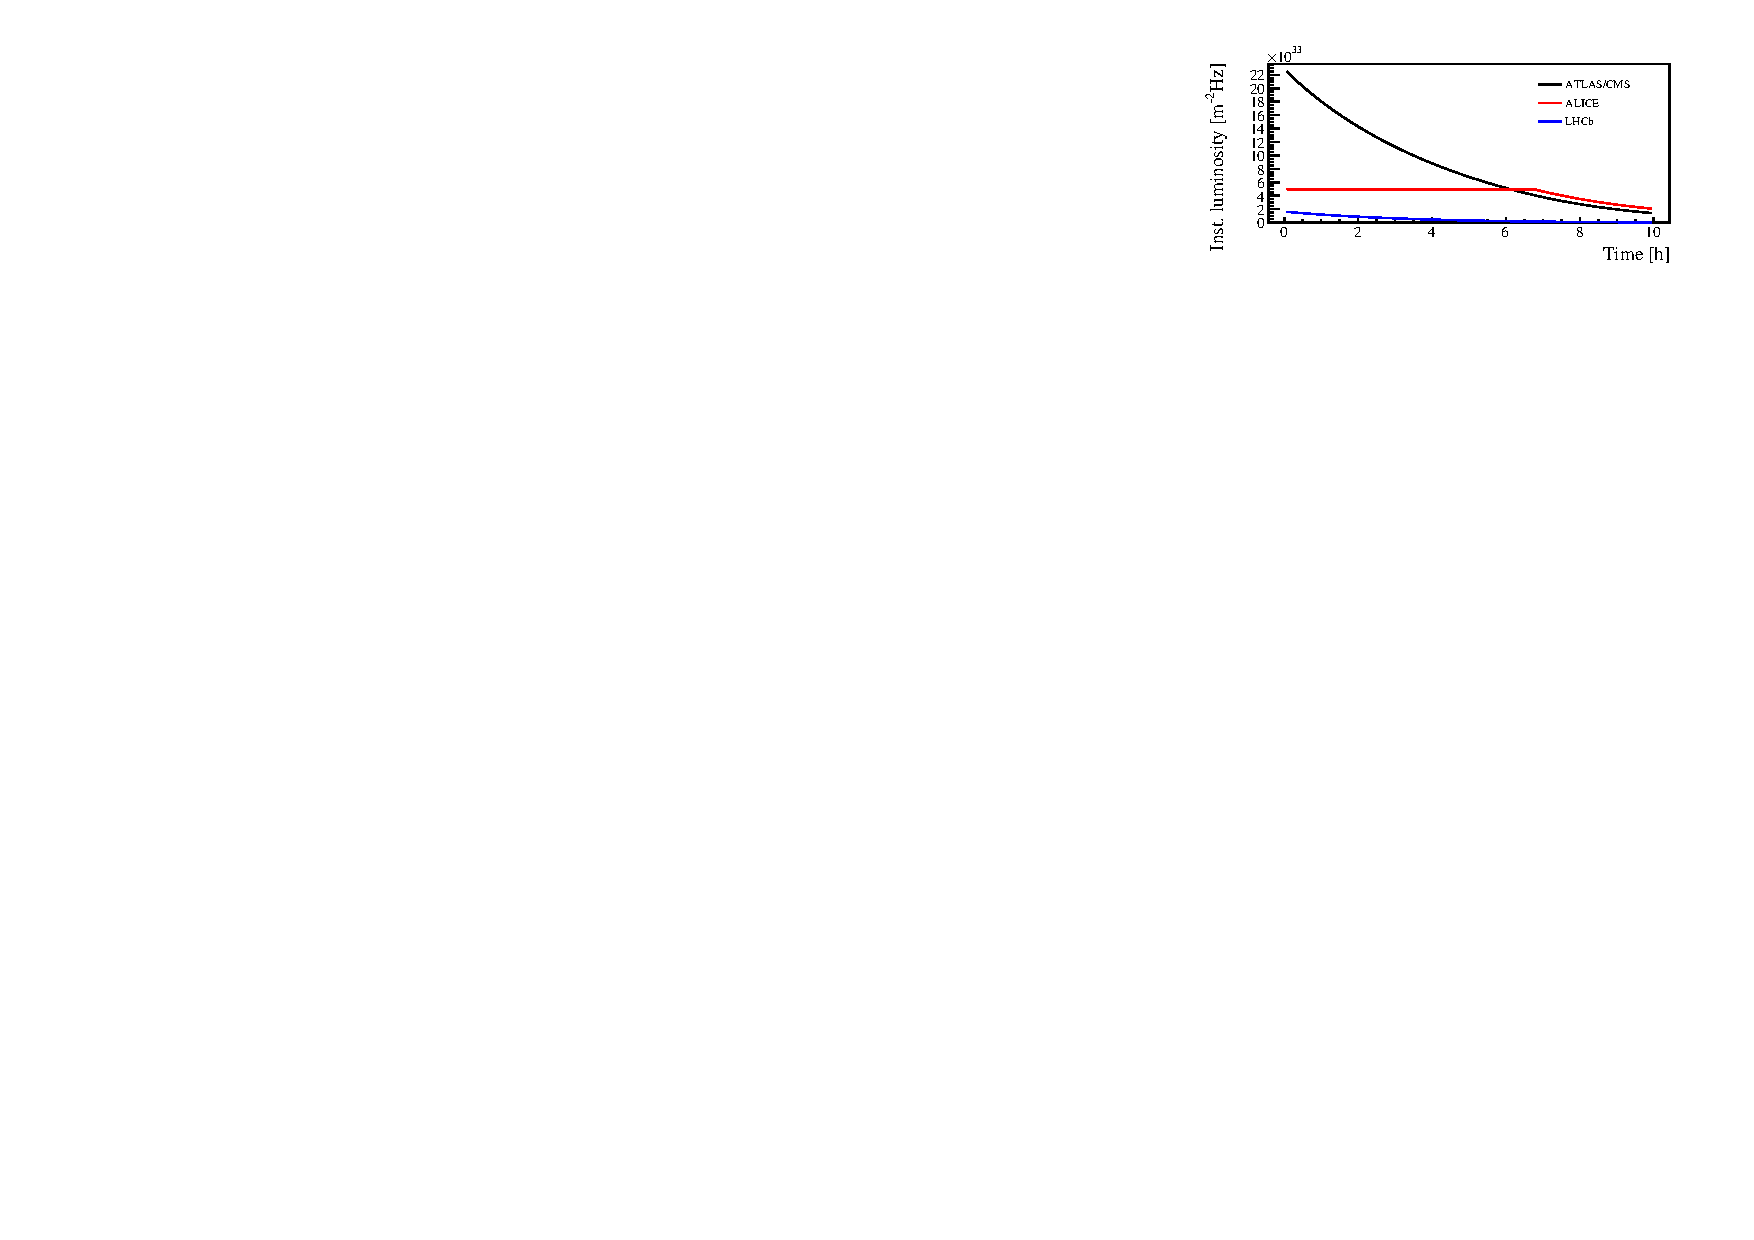
\includegraphics[scale=1.2]{accelerator/p_pb_lumi_evo.pdf} 
\caption{Displayed is the evolution of the instantaneous luminosity in the different IPs. At around \qty{5.4}{h}, the interlock BPM threshold should be reached limiting the fill length to this duration.}
\label{fig:p_pb_lumi_evo}
\end{figure}
At around $\qty{5.4}{h}$, the bunch intensity of the bunches colliding in ATLAS, ALICE and CMS drop below the interlock BPM threshold ultimately limiting the fill length. Key results from the beam evolution study are listed in Tab.~\ref{tab:p_Pb_table}. The expected peak luminosity in ATLAS and CMS is at around $\mathcal{L}_\mathrm{AA}=\qty{22.5\times 10^{29}}{cm^{-2}s^{-1}}$, i.e., roughly a factor $2.5$ larger than in 2016. The integrated luminosity in ATLAS and CMS are expected to approach $\qty{1}{pb^{-1}}$ outperforming the 2016 integrated luminosity by a rough factor $5$. Since the nominal \mbox{HL-LHC} normalised proton emittance of $\epsilon_N=\qty{2.5}{\mu m}$ is assumed, the actual performance may exceed these predictions since normalised proton emittances in the range of $\epsilon_N=\qty{1.3}{\mu m}$ have already been achieved.
\begin{table}[htb]
    \centering
%\begin{tabular}{m{4.5cm}|cccc}
\begin{tabular}{l|ccc}
%\hline                   
%  Quantity                                  & & & & \\
  \hline
Species                                     &\multicolumn{1}{c}{p} & \multicolumn{2}{c}{Pb} \\
\hline
Beam energy \qty{E[Z}{TeV]}                 & \multicolumn{3}{c}{7} \\
Collision energy \qty{\sqrt{\sNN}}{[TeV]}   & \multicolumn{3}{c}{8.78}  \\
Bunch intensity \qty{N_b}{[10^8]}           &\multicolumn{1}{c}{300} &\multicolumn{2}{c}{1.8} \\
No,\ of bunches $k_b$                       &\multicolumn{1}{c}{1232} &\multicolumn{2}{c}{1232} \\
Norm. emittance \qty{\epsilon_N}{[\mu m]}   &\multicolumn{1}{c}{2.5} &\multicolumn{2}{c}{1.65}  \\
Bunch length \qty{\sigma_{z}}{[m]}          &\multicolumn{1}{c}{0.09} &\multicolumn{2}{c}{0.08} \\
Fill time \qty{t_\mathrm{fill}}{h]}         & \multicolumn{3}{c}{5.4} \\
\hline
IP                                          & ATLAS/CMS & ALICE & LHCb \\
\hline
\qty{\bstar}{[m]}                           & 0.5 &  0.5 &  0.5\\
Colliding bunches  $k_c$                    & 1136 & 1120 &  81 \\
Luminosity \qty{\LAA}{[10^{29}cm^{-2}s^{-1}]}               & 22.5 & 5.0 & 1.6  \\
NN luminosity \qty{ \LNN}{[10^{31} {cm}^{-2} {s}^{-1}]}     & 46.8 & 10.4 & 3.3  \\
$\int _{\text{month}}L_{\text{AA}}\text{ dt}$ [nb${}^{-1}$] & 1089 & 416 & 66  \\
$\int _{\text{month}}L_{\text{NN}}\text{ dt}$ [pb${}^{-1}$] & 226 & 87 & 14  \\
 \hline
\end{tabular}
    \caption{The table contains the key parameters and results of the p--Pb beam evolution calculation. A turn-around time, i.e., the time between Beam Dump and Stable Beams, of \qty{2.5}{h} and an operational efficiency factor of $0.5$ is assumed. The final result was scaled down by additional $\qty{5}{\%}$ to take potential deviations of the proton filling pattern into account. The time the first bunches need to reach the interlock BPM threshold is used as the fill time.}
    \label{tab:p_Pb_table}
\end{table}
\subsection{Colliding lighter nuclei at HL-LHC} \label{sec:lightions}
 

The bunch intensity limits in the injectors depend largely on the ion charge which changes at the various stripping stages which must be optimised for space-charge limits, intra-beam scattering, efficiency of electron-cooling,   beam losses on residual gas and other effects in the ion source, Linac4,  LEIR, the PS and SPS.  
Given the uncertainties, the deliverable intensity for other species can only be determined after sufficient time spend commissioning and empirically optimising the many parameters and operating modes of the whole injector chain. 
To simplify present considerations, we postulate a simple form relating the number of ions per bunch, \Nb, to the well-established value
(\Nb(82,208)=\enum{1.9}{8}) for Pb beams  
\begin{equation}
{\Nb}(Z,A)   = {\Nb}(82,208){\left( {\frac{Z}{{82}}} \right)^{ - p}} 
\label{eq:pscaling}
\end{equation}
Fitting such an expression to the limited information~\cite{Manglunki:2016qzl} from the few species used for SPS fixed-target in recent years (since the commissioning of the present ECR ion source and LEIR) yields a value of the fit parameter \(p=1.9\).    
Beam quality requirements for fixed-target beams are, of course, less stringent than for injection into the collider.
Fitting to the first commissioning of Xe beams for the LHC~\cite{Schaumann:2018qat}, on the other hand, gives a much less optimistic \(p=0.75\).   
Although this was the only occasion where any other species than Pb was delivered to the collider, only the simplest version of the injection scheme was used and it is clear that, 
given time, significantly higher intensities could be achieved.  
We consider that  \(1.5\le p\le 1.9\) corresponds to a representative range of possibilities that could be 
realised in fully-prepared future operation.  


In addition, we make a number of simplifying assumptions to allow a simplified, yet meaningful, comparison between species 
\begin{itemize}
    \item  The     \emph{geometric} transverse beam emittances at the start of collisions will be equal to those of Pb beams~\cite{HLLHCPbPbspec}.
    This is justified, at least at the level of the LHC, since the scaling of intra-beam scattering with \(\Nb\), \(Z\) and \(A\), 
    given by  the parameter 
    $f_{\text{IBS}}\text{/(m Hz)}$  
    is generally smaller than for \Pb\ as long as 
    $p\lsim1.9$.  A similar scaling should hold in the injectors such as the SPS where intra-beam scattering may also blow up the emittances.  
    This ignores possible space-charge limits in the injectors which
    should also be considered once the appropriate stripping schemes and charge states have been defined. 
    
    \item Same filling scheme with \(k_c=\)
    \item No luminosity-levelling in any experiment.
     \item Fill length optimised for intensity evolution dominated by luminosity burn-off. 
     \item Equal operational efficiency of 50\%.     Following conventional practice for HL-LHC, the integrated luminosity for a 1-month run is estimated assuming back-to-back ideal fills of optimal length and a turn-around time of \qty{2.5}{h} between the end  of one fill and the resumption of ``Stable Beams''  for collisions in the next.
\end{itemize} 
The parameters are estimated using analytical approximations unlike the more elaborate simulations used in Section~\ref{sec:HLPbPb}.  
Together with the assumption that there is no luminosity levelling, these lead to a higher estimate of integrated luminosity in a one-month run.  
Nevertheless they can be used as a guide to the relative gain factors in integrated nucleon-nucleon luminosity by changing from Pb to a lighter nucleus. 

\begin{table}%% Table from HL-LHC species.nb for p=1.5 
\centering
{\small
	\begin{tabular}{|*{1}{*{7}{|l}|}|}
\speciesheader\\
\hline
$\gamma$                                                                       &  \(3760.\) & \(3390.\) & \(3760.\) & \(3470.\) & \(3150.\) & \(2960.\) \\
$\sqrt{s_{\text{NN}}}\text{/TeV}$                                              &  \(7.\) & \(6.3\) & \(7.\) & \(6.46\) & \(5.86\) & \(5.52\) \\
$\sigma _{\text{had}}\text{/b}$                                                &  \(1.41\) & \(2.6\) & \(2.6\) & \(4.06\) & \(5.67\) & \(7.8\) \\
$\sigma _{\text{BFPP}}\text{/b}$                                               &  \(2.36\times 10^{-5}\) & \(0.00688\) & \(0.0144\) & \(0.88\) & \(15.\) & \(280.\) \\
$\sigma _{\text{EMD}}\text{/b}$                                                &  \(0.0738\) & \(1.24\) & \(1.57\) & \(12.2\) & \(51.8\) & \(220.\) \\
$\sigma _{\text{tot}}\text{/b}$                                                &  \(1.48\) & \(3.85\) & \(4.18\) & \(17.1\) & \(72.5\) & \(508.\) \\
$N_b$                                                                          &  \(6.24\times 10^9\) & \(1.85\times 10^9\) & \(1.58\times 10^9\) & \(6.53\times 10^8\) & \(3.56\times 10^8\) & \(1.9\times 10^8\) \\
$\epsilon _{\text{xn}}\text{/$\mu $m}$                                         &  \(2.\) & \(1.8\) & \(2.\) & \(1.85\) & \(1.67\) & \(1.58\) \\
$f_{\text{IBS}}\text{/(m Hz)}$                                                 &  \(0.0662\) & \(0.0894\) & \(0.105\) & \(0.13\) & \(0.144\) & \(0.167\) \\
$W_b\text{/MJ}$                                                                &  \(68.9\) & \(45.9\) & \(43.6\) & \(32.5\) & \(26.5\) & \(21.5\) \\
$L_{\text{AA0}}/\text{cm}^{-2}s^{-1}$                                          &  \(1.46\times 10^{31}\) & \(1.29\times 10^{30}\) & \(9.38\times 10^{29}\) & \(1.61\times 10^{29}\) & \(4.76\times 10^{28}\) & \(1.36\times 10^{28}\) \\
$L_{\text{NN0}}/\text{cm}^{-2}s^{-1}$                                          &  \(3.75\times 10^{33}\) & \(2.06\times 10^{33}\) & \(1.5\times 10^{33}\) & \(9.79\times 10^{32}\) & \(7.93\times 10^{32}\) & \(5.88\times 10^{32}\) \\
$P_{\text{BFPP}}\text{/W}$                                                     &  \(0.0031\) & \(0.179\) & \(0.303\) & \(5.72\) & \(43.4\) & \(350.\) \\
$P_{\text{EMD1}}\text{/W}$                                                     &  \(4.98\) & \(16.5\) & \(16.9\) & \(40.5\) & \(76.7\) & \(141.\) \\
$\tau _{\text{L0}}\text{/h}$                                                   &  \(16.4\) & \(21.3\) & \(23.\) & \(13.5\) & \(5.87\) & \(1.57\) \\
$T_{\text{opt}}\text{/h}$                                                      &  \(9.04\) & \(10.3\) & \(10.7\) & \(8.23\) & \(5.42\) & \(2.8\) \\
\qty{\left\langle L_{\text{AA}}\right\rangle}{cm^{-2}s^{-1}}             &  \(8.99\times 10^{30}\) & \(8.34\times 10^{29}\) & \(6.17\times 10^{29}\) & \(9.46\times 10^{28}\) & \(2.23\times 10^{28}\) & \(3.8\times 10^{27}\) \\
$\left\langle L_{\text{NN}}\text{$\rangle $/}\text{cm}^{-2}s^{-1}\right.$      &  \(2.3\times 10^{33}\) & \(1.33\times 10^{33}\) & \(9.87\times 10^{32}\) & \(5.76\times 10^{32}\) & \(3.71\times 10^{32}\) & \(1.64\times 10^{32}\) \\
$\int _{\text{month}}L_{\text{AA}}\text{ dt/}\text{nb}^{-1}$                   &  \(1.17\times 10^4\) & \(1080.\) & \(799.\) & \(123.\) & \(28.9\) & \(4.92\) \\
$\int _{\text{month}}L_{\text{NN}}\text{ dt/}\text{pb}^{-1}$                   &  \(2980.\) & \(1730.\) & \(1280.\) & \(746.\) & \(481.\) & \(213.\) \\
$R_{\text{had}}\text{/kHz}$                                                    &  \(2.07\times 10^4\) & \(3340.\) & \(2440.\) & \(653.\) & \(270.\) & \(106.\) \\
$\mu$                                                                          &  \(1.64\) & \(0.266\) & \(0.194\) & \(0.0518\) & \(0.0215\) & \(0.00842\) \\
\end{tabular}

	}
   \caption{Parameters and performance for a range of light nuclei with a moderately optimistic value of the scaling parameter \(p=1.5\) in \eqref{eq:pscaling}. }
\end{table}
%\vspace{1em}


\begin{table}%% Table from HL-LHC species.nb for p=1.5 
\centering
{\small
	\begin{tabular}{|*{1}{*{7}{|l}|}|}
\speciesheader\\
\hline$\gamma$                                                                       &    \(3760.\) & \(3390.\) & \(3760.\) & \(3470.\) & \(3150.\) & \(2960.\) \\
$\sqrt{s_{\text{NN}}}\text{/TeV}$                                              &    \(7.\) & \(6.3\) & \(7.\) & \(6.46\) & \(5.86\) & \(5.52\) \\
$\sigma _{\text{had}}\text{/b}$                                                &    \(1.41\) & \(2.6\) & \(2.6\) & \(4.06\) & \(5.67\) & \(7.8\) \\
$\sigma _{\text{BFPP}}\text{/b}$                                               &    \(2.36\times 10^{-5}\) & \(0.00688\) & \(0.0144\) & \(0.88\) & \(15.\)& \(280.\) \\
$\sigma _{\text{EMD}}\text{/b}$                                                &    \(0.0738\) & \(1.24\) & \(1.57\) & \(12.2\) & \(51.8\) & \(220.\) \\
$\sigma _{\text{tot}}\text{/b}$                                                &    \(1.48\) & \(3.85\) & \(4.18\) & \(17.1\) & \(72.5\) & \(508.\) \\
$N_b$                                                                          &    \(1.58\times 10^{10}\) & \(3.39\times 10^9\) & \(2.77\times 10^9\) & \(9.08\times 10^8\) & \(4.2\times 10^8\) & \(1.9\times 10^8\) \\
$\epsilon _{\text{xn}}\text{/$\mu $m}$                                         &    \(2.\) & \(1.8\) & \(2.\) & \(1.85\) & \(1.67\) & \(1.58\) \\
$f_{\text{IBS}}\text{/(m Hz)}$                                                 &    \(0.168\) & \(0.164\) & \(0.184\) & \(0.18\) & \(0.17\) & \(0.167\) \\
$W_b\text{/MJ}$                                                                &    \(175.\) & \(84.3\) & \(76.6\) & \(45.2\) & \(31.4\) & \(21.5\) \\
$L_{\text{AA0}}/\text{cm}^{-2}s^{-1}$                                          &    \(9.43\times 10^{31}\) & \(4.33\times 10^{30}\) & \(2.9\times 10^{30}\) & \(3.11\times 10^{29}\) & \(6.66\times 10^{28}\) & \(1.36\times 10^{28}\) \\
$L_{\text{NN0}}/\text{cm}^{-2}s^{-1}$                                          &    \(2.41\times 10^{34}\) & \(6.93\times 10^{33}\) & \(4.64\times 10^{33}\) & \(1.89\times 10^{33}\) & \(1.11\times 10^{33}\) & \(5.88\times 10^{32}\) \\
$P_{\text{BFPP}}\text{/W}$                                                     &    \(0.0199\) & \(0.601\) & \(0.935\) & \(11.\) & \(60.6\) & \(350.\) \\
$P_{\text{EMD1}}\text{/W}$                                                     &    \(32.\) & \(55.6\) & \(52.2\) & \(78.3\) & \(107.\) & \(141.\) \\
$\tau _{\text{L0}}\text{/h}$                                                   &    \(6.45\) & \(11.6\) & \(13.1\) & \(9.74\) & \(4.96\) & \(1.57\) \\
$T_{\text{opt}}\text{/h}$                                                      &    \(5.68\) & \(7.62\) & \(8.08\) & \(6.98\) & \(4.98\) & \(2.8\) \\
$\left\langle L_{\text{AA}}\text{$\rangle $/}\text{cm}^{-2}s^{-1}\right.$      &    \(4.54\times 10^{31}\) & \(2.45\times 10^{30}\) & \(1.69\times 10^{30}\) & \(1.68\times 10^{29}\) & \(2.95\times 10^{28}\) & \(3.8\times 10^{27}\) \\
$\left\langle L_{\text{NN}}\text{$\rangle $/}\text{cm}^{-2}s^{-1}\right.$      &    \(1.16\times 10^{34}\) & \(3.93\times 10^{33}\) & \(2.71\times 10^{33}\) & \(1.02\times 10^{33}\) & \(4.91\times 10^{32}\) & \(1.64\times 10^{32}\) \\
$\int _{\text{month}}L_{\text{AA}}\text{ dt/}\text{nb}^{-1}$                   &    \(5.89\times 10^4\) & \(3180.\) & \(2190.\) & \(218.\) & \(38.2\) & \(4.92\) \\
$\int _{\text{month}}L_{\text{NN}}\text{ dt/}\text{pb}^{-1}$                   &    \(1.51\times 10^4\) & \(5090.\) & \(3510.\) & \(1330.\) & \(636.\) &\(213.\) \\
$R_{\text{had}}\text{/kHz}$                                                    &    \(1.33\times 10^5\) & \(1.12\times 10^4\) & \(7540.\) & \(1260.\) & \(378.\) & \(106.\) \\
$\mu$                                                                          &    \(10.6\) & \(0.893\) & \(0.598\) & \(0.1\) & \(0.03\) & \(0.00842\) \\
\end{tabular}

	}
   \caption{Parameters and performance for a range of light nuclei with an optimistic value of the scaling parameter \(p=1.9\) in \eqref{eq:pscaling}. }
\end{table} 
 
 Collimation \cite{Hermes:2016axvg}

\subsection{Short run for \pO}
\label{sec:pOrun} %% Hans Dembinski can refer to this section  

As discussed in Section~
\ref{sec:pOcosmic}, a  short \pO\ collision run is of interest for cosmic-ray physics.  
This could be scheduled with rapid set-up in LHC on the successful 
model of the 2012 \pPb\ run\cite{} 
which was later re-used in the 
2017 \XeXe\ run\cite{Schaumann:2018qat}.  
Each of those runs took  about 16~h of LHC operation time, 
including set-up and physics data-taking. 

Because oxygen is used as the carrier gas in the CERN heavy-ion source, 
the idea has been mooted that 
it may be possible to switch from \Pb\ to
\isotope{16}{O}{8+}  beams for the LHC, and back,  
somewhat more rapidly than other species.  
However it appears that the process is still not quick enough to allow, say, 
a short p--O run at the end of one of the annual Pb-Pb runs.  
A more practical possibility would be to schedule the run 
earlier in the year in order to provide time for 
the source to be switched back to Pb operation
afterwards for the one-month run later in the year.   
Commissioning of the O beam in the injectors for single-bunch injection into the LHC
would need to be scheduled in parallel with p-p operation in the weeks before the \pO\ run. 

To keep the LHC commissioning time on the order of 8~h, as in the 2017 Xe--Xe run,  
the total charge per beam should be limited to similar values.  
This would lead to a filling scheme with 
\(\simeq 10\)~bunches. 
A  probable disadvantage of this scheme is that the \pO\  run 
would have to be done with the currently operational \pp\ optics with    \bstarval{10}, at IP2, rather than  \bstarval{0.5} as would be typical of an optics set up for heavy-ion operaion.  
This would mean that the ALICE experiment would receive less integrated luminosity than ATLAS and CMS, 
as  occurred in the 2017 \XeXe\ run~\cite{Schaumann:2018qat}.

\subsection{Heavy-ion performance of HE-LHC} 
% John and Michaela

For the moment assume same injected beams as HL-LHC 
in the absence of work on 
further possible upgrades to the injectors. 

Arguments from FCC Week in Amsterdam. 
Modest factor in integrated luminosity.

BFPP power with Pb very high. 
Could be alleviated with lighter species.
Expect roughly similar species scaling to HL-LHC in Section~\ref{sec:lightions}.


\end{document}
